
% Due Date: 6/6/14

\chapter{Introduction}
\label{chapter:intro}

The rate of progress of science and
engineering is tied to the ability of scientists and
engineers to conduct experiments. In the past several decades,
the advent of computers and the increasing cost and complexity of 
actual experiments has motivated many scientists to conduct 
research via computational methods. The large and growing 
number of computational scientists has been a core driver 
behind the consistent improvement of the world's supercomputers. 
Figure~\ref{fig:supergrowth} shows the progression of 
performance capabilities of the world's top 500 supercomputers 
over time \cite{Top500}. The steady march of performance 
improvements is indicative of the increasing importance 
that is placed on computational science and engineering. 

\begin{figure}[ht]
\centering
\includegraphics[scale=0.5]{figs/top500.jpg}
\caption{Peak Performance of the Top 500 Supercomputers\cite{Top500}\label{fig:supergrowth}}
\end{figure}

Despite the growing importance of supercomputing to the
progress of science and engineering, the programming tools available
for conducting computational science are relatively primitive.
The same programming systems that were developed at 
the dawn of supercomputing are still in use today even
though hardware performance has increased by many orders
of magnitude (note the logarithmic scale in 
Figure~\ref{fig:supergrowth}). Furthermore, the performance
improvements of modern hardware have only been made
possible through the deployment of increasingly
complex and exotic architectures.
Consequently, the burden of fully leveraging the 
computational power of current supercomputers is
shouldered directly by computational scientists who are 
ill-equipped to handle the mounting complexity.

The obvious solution to this problem, as with most
complex problems in computer science, is abstraction.
Extracting the full potential from modern and future
supercomputers requires the development of new programming
models with the necessary abstractions to simplify programming 
while still achieving high performance and easing the 
costs of porting and tuning important scientific codes. 
In this thesis we present Legion, a new programming model 
and runtime system based on the abstraction of logical regions
as one solution for programming current and future distributed
heterogeneous supercomputers. 

\section{Dissertation Overview}
\label{sec:overview}

The design and implementation of the Legion programming
system has many different layers of abstraction to address
the multitude of problems associated with modern supercomputing.
The remainder of this chapter is dedicated to 
providing a detailed description of our motivation for Legion 
and the design principles used to guide our decision making
when developing the necessary abstractions. 

The technical discussion of Legion begins in Chapter~\ref{chapter:model}
by introducing logical regions as the fundamental abstraction 
and describes the resulting programming model built 
with logical regions as the foundation.
Chapter~\ref{chapter:arch} initiates our description of the
implementation of the Legion runtime system by covering
the architecture of the different layers of the system. 
Chapters~\ref{chapter:logical}-\ref{chapter:garbage} cover
the details of the Legion runtime implementation including traversals
of the logical and physical region trees, the distribution
of meta-data structures, and garbage collection. 
Chapter~\ref{chapter:mapping} introduces Legion's novel
mapper interface and illustrates how mappers can be
used to intelligently tune applications for different
machine architectures. In Chapters~\ref{chapter:relaxed}
and \ref{chapter:resilience} we show two important
extensions to Legion that add both expressivity and 
resiliency to the programming system. In 
Chapter~\ref{chapter:s3d} we demonstrate that Legion
is a real system, capable of handling S3D, a production
combustion simulation. Finally, we give a detailed
accounting of related work in Chapter~\ref{chapter:related}
and draw conclusions in Chapter~\ref{chapter:conclusion}.

\section{The State of Programming Supercomputers}
\label{sec:programming}

Supercomputers have a long history of being some of
the most challenging machines to program. Before 
delving into the details of Legion, we first investigate
the state of programming modern supercomputers to
discover the origins of many of the problems faced
by today's computational scientists.  While there are many 
approaches to programming supercomputers, we cover
only the most common ones here.  A more complete description
of related work and other programming systems for
supercomputers can be found in Chapter~\ref{chapter:related}.

By far, the most ubiquitous programming system
in use for programming supercomputers today is
the Message Passing Interface (MPI) standard \cite{MPI}.
MPI is a Singe-Program Multiple-Data (SPMD) programming model
where many copies of the application are run in 
parallel to operate on different sets of data.
MPI provides a uniform interface for performing
communication between multiple processes running
on different nodes of a supercomputer by sending
messages. Additionally, it also provides support
for performing low-latency synchronization such
as barriers and collective operations. The MPI
interface is designed to be general enough that it
can be implemented on top of many different 
interconnects including Ethernet, Infiniband,
Cray Gemini and Aires, and IBM Blue Gene. This
approach makes it possible to migrate
MPI codes to new machine architectures.

While MPI provides a universal interface for 
programming supercomputers, it suffers from a
fundamental flaw that both impedes its performance
portability and compromises its ability to support 
modular code, thus resulting in applications that are
inherently difficult to maintain. Consider the following 
example MPI pseudo code which illustrates the posting of
an asynchronous receive followed by some anonymous
work {\tt Y} before using the received results:
\begin{verbatim}
receive(x, ...);
Y;
sync;
f(x);
\end{verbatim}
This pseudo code represents a common MPI idiom. In
order to hide the latency of communication, MPI
applications must use asynchronous sends and 
receives to overlap communication with additional
work (e.g. {\tt Y}). This leads to two problems.
\begin{enumerate}
\item It is the responsibility of the programmer
      to find the useful computation {\tt Y} to
      overlap with the {\tt receive}. There are
      several constraints on this choice of {\tt Y}.
      The execution of {\tt Y} must not be too short
      or the latency of the {\tt receive} will not
      be hidden, and it must not be too long or the
      continuation {\tt f(x)} will be unnecessarily
      delayed. Thus, for each new target machine the
      choice of {\tt Y} will have to be re-tuned for 
      the communication latency of the underlying
      interconnect. Furthermore, on 
      machines with dynamically routed interconnect
      networks \cite{CrayGemini}, it will be impossible
      for programmers to accurately determine a
      choice for {\tt Y} as it will vary dynamically 
      both in space and time with the load on the network.
\item Since {\tt Y} is not permitted to use {\tt x},
      {\tt Y} must be an unrelated computation, resulting
      in code which is inherently non-modular. Being
      able to construct modular code is a fundamental 
      pillar of software engineering and a crucial
      tool in creating abstractions that manage
      software complexity. MPI requires 
      programmers to destroy modularity for the
      sake of performance, ultimately resulting in code 
      that is difficult to maintain and refactor.
\end{enumerate}
These deficiencies permeate many of the applications
that use MPI today, resulting in codes which are inherently
difficult to maintain and not performance portable. In
Chapter~\ref{chapter:model} we will demonstrate how Legion's
programming model is capable of automatically overlapping
computation with communication in a way that still
permits and encourages modular code.

While MPI is the primary programming system used
for communicating between nodes, programmers
use additional tools for extracting performance
within a node. Most frequently, programmers use 
OpenMP \cite{OPENMP98} to take advantage of loop-level
data parallelism. The OpenMP runtime maintains
a set of background threads which are used for
executing parallel loops. Programmers are responsible
for annotating parallel loops with pragma statements
that detail how loops should be parallelized. While
this approach benefits from its simplicity, it too
is fundamentally flawed. OpenMP is ignorant of cache
hierarchies and non-uniform memory access (NUMA)
domains, resulting in code with sub-optimal 
performance. Furthermore, OpenMP is only capable of 
distributing work across the homogeneous CPU processors 
in a blocking fashion, making it impossible to offload 
work from other loops in parallel onto accelerators. In 
Chapter~\ref{chapter:mapping} we will show how the 
Legion mapping interface allows tasks to run in 
parallel across both CPUs and GPUs simultaneously 
while also allowing mappings that are both cache- and NUMA-aware.

To target accelerators most programmers use either
CUDA \cite{CUDA} or OpenCL \cite{Khronos:OpenCL}. Both 
CUDA and OpenCL provide the necessary primitives for
copying data between the various memories (e.g.
framebuffer and system memory) as well as the
ability to execute kernels on the accelerator
cores. While these languages are sufficient for programming
accelerators, they place a significant burden
on the programmer. Programmers are responsible
for issuing the explicit (asynchronous)
data movement commands and then properly
synchronizing these data movements with 
computation using either streams in CUDA or
events in OpenCL. Much like MPI, this again
places the burden of overlapping computation
with data movement on the programmer and 
also makes it easy to introduce complex
synchronization bugs. Furthermore, the
data movement operations for CUDA and OpenCL
do not compose with the operations in MPI,
commonly requiring the data first be moved
to a node with an MPI communication primitive 
and then later moved again with a CUDA or
OpenCL call. Synchronizing between all of 
these different operations because of interface
incompatibility adds latency and increases 
code complexity. 

Due to the programming challenges inherent
in using CUDA and OpenCL, recently OpenACC \cite{OpenACC}
has been proposed as a way to use accelerators 
with a model similar to OpenMP. To use OpenACC
programmers also annotate loops with 
pragmas much like OpenMP.  In addition
to specifying how to parallelize the loop, 
programmers must also specify the data allocations
that will be accessed. In some respects 
this is a positive step as it is the first instance 
of a programming system being aware of the 
structure of program data. By leveraging this
knowledge, OpenACC can automatically move
data between system memory and the GPU framebuffer
memory. However, OpenACC fails to fully understand
the data dependences between consecutive loops
and by default always copies data both down
and back from the GPU for each loop. Programmers
can address this performance problem by adding
additional annotations stating which data
can be left on the GPU and which data can
be released without copying it back. However,
incorrect annotations or code refactoring
can easily introduce bugs which the
programming system can neither detect nor fix.

As a whole, these programming systems constitute
an eclectic collection of tools with little
common infrastructure and vastly different semantics.
Scientific programmers are forced to choose
a subset of these tools that match their target
machine and then provide the considerable glue logic
for mediating between the various APIs and programming
models. Writing this glue code is both tedious and 
error-prone, ultimately adding unnecessary complexity 
to applications which are already extremely sophisticated. 
It is obvious that this ad hoc approach to programming 
supercomputers is neither ideal nor scalable and 
therefore new approaches must be found.

\section{Motivation}
\label{sec:motivation}

Our motivation in designing Legion is not simply to fix
the problems of current programming systems outlined in
the previous section, but rather to construct a system
that meets the needs of programmers for both modern and
future supercomputing architectures. To meet this 
constraint, the design of Legion is based on three 
important and noticeable trends in supercomputing that
forecast the future of the field: the increasing cost 
of data movement relative to the cost of computation, 
the increasing amount of dynamism in both hardware and 
software, and the growing prevalence of heterogeneity 
of both processors and memories. We now discuss each of
these trends in turn.

\subsection{Cost of Data Movement}
\label{subsec:movement}

While the peak floating point throughput of modern supercomputers
has continued to scale with Moore's law, the maximum
theoretical bandwidth provided by both memory and communication
interfaces has scaled linearly at best. Figure~\ref{fig:moore}
and Figure~\ref{fig:memband} \cite{CUDA} show the theoretical 
peak floating point and bandwidth throughput trends respectively
for both CPUs and GPUs over time. The growing disparity between
compute throughput and bandwidth is driving more applications
to be limited by the cost of data movement (either in terms
of performance or power). In the future only the most computationally
expensive applications (e.g. matrix multiply) will remain 
limited by compute throughput.

In addition to the disparity between compute throughput and
bandwidth, the latency of communication is continuing to grow.
As machines increase in size, the cost of communicating 
between nodes also increases. This trend is irreversible as the
latency of communication will always be fundamentally limited 
by the speed of light.

Consequently, the cost of data movement is
quickly coming to dominate the performance of most 
scientific computing applications. Also, since data movement
is one of the more expensive operations in terms
of power for hardware, these costs extend beyond raw
execution time, and further into the power budgets of
modern hardware. 

\begin{figure}[ht]
\centering
\subfloat[Peak Theoretical Floating Point Throughput]{
\label{fig:moore}
\includegraphics[scale=0.35]{figs/moore.png}
}
\subfloat[Peak Theoretical Memory Bandwidth]{
\label{fig:memband}
\includegraphics[scale=0.35]{figs/memband.png}
}
\caption{Comparing Peak Floating Point and Bandwidth Performance\cite{CUDA}\label{fig:peak}}
\end{figure}

\subsection{Hardware and Software Dynamism}
\label{subsec:dynamism}

Another important trend is the burgeoning amount of 
dynamism present in both software and hardware. Initially 
most scientific computations operated on structured
Cartesian grids. However, recent scientific 
applications are coming to operate on more irregular
data structures such as graphs \cite{Pennant13}
and unstructured meshes \cite{Liszt11}. These
applications construct data structures at runtime
to match the input data on which they are going to
operate. Being able to support these kinds of applications
requires programming systems capable of handling dynamic
partitioning and mapping of both data and tasks. 

Even more dynamic are applications that perform
operations such as Adaptive Mesh Refinement (AMR)
 \cite{BoxLib,Chombo}. These codes react to changes
in the simulation to create new simulation spaces
and computations. Handling these applications requires
the ability to dynamically re-balance both data and
task distributions at runtime throughout the
execution of the application. These kinds of applications
are becoming more prevalent and require programming
systems capable of reacting to their dynamism.

In addition to the dynamism of emerging software, hardware
is also becoming more dynamic. The most obvious 
evidence of dynamism in hardware is the presence of dynamically
routed interconnect networks that leverage on-line
routing algorithms based on traffic flow \cite{CrayGemini}
which adds variability to the latencies of communication.
More subtly, the strict power budgets of future 
architectures will introduce hardware with low-power
cores \cite{Tegra} and support for dark silicon \cite{DarkSilicon11}. 
Finally, as circuit feature sizes continue to shrink, the 
prevalence of hardware faults, both soft and hard, will make 
hardware less reliable, requiring dynamic recovery mechanisms.

%The increasing dynamism of both software and hardware
%signaled a clear need for Legion to be formulated as
%a runtime system capable of performing all of its
%operations dynamically. While this did not preclude 
%the development of more common static programming
%system components such as a programming language and
%compiler, it did drive us to make the runtime system 
%the initial and primary focus of Legion.

\subsection{Heterogeneous Architectures}
\label{subsec:heterogeneous}

The third, and most prominent trend, is the emergence 
of heterogeneous architectures.
The introduction of accelerators into the previously
homogeneous world of supercomputing fundamentally disrupted 
the nature of how supercomputers were both used and
programmed. Accelerators such as NVIDIA 
and AMD GPUs as well as Intel Xeon Phis have greatly
complicated programming models. Accelerators introduce dissonance
in processor speeds by providing additional cores
optimized for throughput instead of latency. Furthermore,
accelerators introduce heterogeneity not just in kinds
of processors, but in kinds of memory as well. For example,
most GPUs require programmers to explicitly manage
the placement and movement of data between framebuffer
memories, zero-copy memories, and on-chip shared memories.
More recently, new kinds of memory are being
proposed for use by both CPUs and GPUs. The incorporation 
of flash memory, non-volatile memory (NVRAM), and 
stacked DRAM will further add to the heterogeneity of
memory hierarchies.

The expanding presence of heterogeneity in system
architectures has presented programmers with the 
daunting challenge of determining the best {\em mapping}
of their applications to the target hardware. A mapping
is simply a determination of how to assign computations
to processors, and how to place data within the
memory hierarchy. In homogeneous systems mappings are generally 
simple: work is evenly divided amongst cores 
with identical performance and data is evenly 
divided between nodes. Heterogeneity opens up many
new degrees of freedom that make 
determining the best mapping significantly more
challenging. To further complicate the problem, mapping
decisions today are usually baked into the source code
as we described in Section~\ref{sec:programming}. Changing 
a mapping routinely requires significant code refactoring, 
including modifications to both data movement and synchronization 
code that can easily introduce correctness bugs. 
For this reason, programmers usually only explore a few 
mappings before settling for sub-optimal performance. 

%As a result of heterogeneity, we determined that 
%Legion should explicitly decouple the specification 
%of an application from how it is mapped onto the
%target architecture. Even more important we determined
%that it is imperative that mapping decisions be
%independent from the correctness of the application,
%thus facilitating both auto-tuning and easy porting of 
%Legion applications to new architectures.

\section{Legion Design Principles}
\label{sec:design}
Our design of Legion is based on both the problems
experienced by current programmers, described
in Section~\ref{sec:programming}, as well as the
motivating trends noted in Section~\ref{sec:motivation}.
The consequence of all these factors is that
current scientific programmers face immense complexity
when implementing their applications. It is therefore
crucial that Legion provide abstractions for
managing this complexity.

To guide our design of Legion abstractions, we 
conceptualized the construction of a scientific 
application as being composed of four primary 
components divided along two axes as shown in 
Figure~\ref{fig:designspace}. On the horizontal axis 
we distinguish between the code written for specifying 
an application in a machine-independent way (e.g. a 
generic algorithm) versus the code used for mapping
the application onto a specific architecture.
On the vertical axis we differentiate between
code used for specifying how an application
should be executed, which we refer to as the 
{\em policy} of an application, from the code 
used to carry out the policy, which we call 
the {\em mechanism} of the application.

\begin{figure}[ht]
\centering
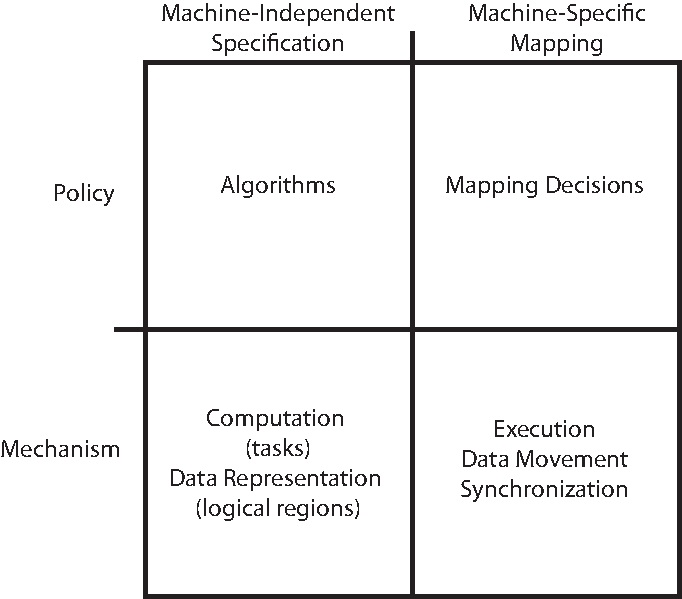
\includegraphics[scale=0.7]{figs/designspace.pdf}
\caption{Components of Supercomputing Applications\label{fig:designspace}}
\end{figure}

Based on this classification of the various
components of an application, we developed
the two design principles on which Legion is
based.  First, mechanism should be decoupled
from policy, and second, applications should
be decoupled from their mapping. These principles
suggest where abstractions should be placed and
serve as the foundation on which the rest
of the Legion architecture is built. Specifically,
the design goal of Legion is two-fold:
\begin{itemize}
\item Decouple mechanism from policy - provide
      abstractions for applications to specify
      algorithms and data partitioning policy,
      while Legion provides the implementation
      of these abstractions (mechanism).
\item Decouple specification from mapping - 
      provide two sets of abstractions: one for
      describing applications independent of
      particular machines (specification)
      and another for describing how an application
      is targeted to a specific architecture (mapping).
\end{itemize}

The scope of Legion and its various 
components can be seen in Figure~\ref{fig:legiondesign}. 
We now detail each of these design principles 
in more detail with regards to how they relate 
to the trends described in Section~\ref{sec:motivation}.

\begin{figure}[ht]
\centering
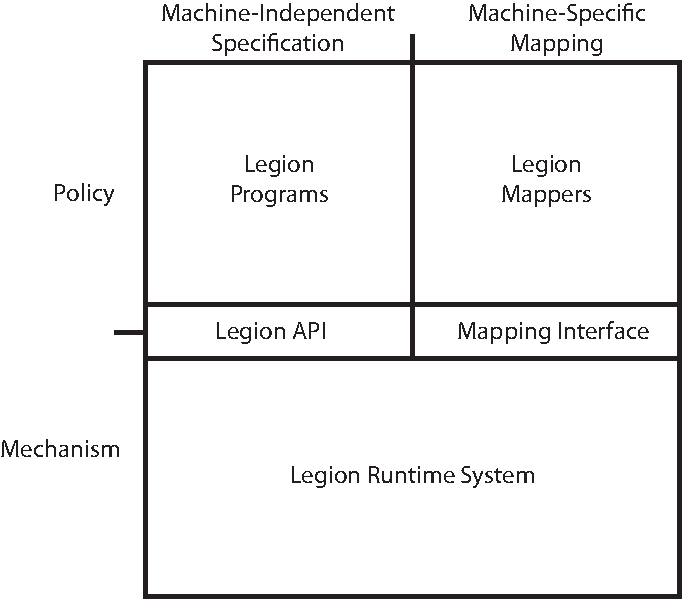
\includegraphics[scale=0.7]{figs/legiondesign.pdf}
\caption{Legion Design Overview\label{fig:legiondesign}}
\end{figure}

\subsection{Decoupling Policy from Mechanism}
\label{subsec:mechanism}
Legion provides an
implementation of the necessary mechanisms
for performing computations, orchestrating
data movement, and engaging in synchronization.
It remains the application developer's
responsibility to specify the policies for
an application including the algorithms to
be used and the mapping of computations and
partitioned data onto the target architecture.

To be more specific,
it is important that Legion applications
be able to select partitioning algorithms
for data because the partitioning strategy is
closely tied to the algorithmic choices that
cannot be made correctly for every application.
On the other hand, it is also important that
Legion carry out the partitioning operation,
both because it relieves the programmer of a
tedious task and also because Legion needs
to know the partitioning of data in order to
carry out other functions. As another example
, Legion applications should be able to map 
tasks onto any processors and data into any 
memories, but Legion should be responsible 
for implementing the necessary mechanisms 
(e.g. copies and synchronization)
for doing this in a way that is consistent
with the application specification.

It is our assertion that this decoupling is
essential to the future of any programming 
system for supercomputers because
of the increasing dynamism and growing 
heterogeneity discussed in Section~\ref{sec:motivation}.
Application codes need to be capable of being
developed without needing to re-implement
data movement, synchronization,
and scheduling routines for each change in
algorithm or target architecture that
appears on the horizon. By decoupling policy
from mechanism we can reduce the amount of
code that programmers need to write 
when changing the structure of applications
for new architectures.

\subsection{Decoupling Specification from Mapping}
\label{subsec:specification}
Our second design principle for Legion is that
applications should be described as 
machine-independent specifications and that 
any decisions required for targeting a particular
architecture should be explicitly decoupled and
specified as part of an application's mapping.
All three of the trends identified in 
Section~\ref{sec:motivation} are drivers of
this design goal. The increasing complexity
of applications and architectures coupled with
increasing cost of data movement is causing
an explosion in the space of
potential mappings of an application. Coupling
the specification of an application with the
mapping fundamentally impedes the exploration
of this space and results in poor performance 
(by any metric, including both performance
and power efficiency).  Unless these two
aspects are explicitly decoupled so that the
search for optimal mappings can be abstracted 
and automated, applications will never be capable 
of achieving peak performance.

Our goal in Legion is therefore 
straightforward: provide a programming system
capable of supporting machine-independent 
specifications of applications and a separate
mechanism for mapping (and re-mapping) specifications 
onto both current and future architectures.
If successful, Legion applications will be both
easy to tune and port to new
machines. To achieve this goal, we will need 
machine-independent abstractions for describing
both computation (tasks) and data (logical
regions), as we discuss in Chapter~\ref{chapter:model}.

\subsection{Legion Non-Goals}
\label{subsec:nongoals}
While we have chosen to tackle several of the
significant problems facing supercomputing, we are
not claiming to solve all such problems. Specifically, 
there are two problems which we are not attempting to 
solve: the determination of the best mapping and programmability. 

We have avoided having Legion implement any
policy decisions and have instead insured that
all policy decisions are explicitly exposed 
either to the application or the mapper. The
reason for this is simple: we do not believe
that it is possible for any programming system
to always make the ideal policy decisions for the cross-product
of all application codes with all target architectures.
Instead, Legion lets applications and mappers 
decide what the important policy decisions are 
for each of their specific domains without any 
interference from Legion. More importantly, we have 
exposed these decisions in a disciplined way that 
organizes policy decisions into application policies 
and mapping policies, allowing developers to address 
them independently.

A difficulty with exposing all policy decisions is
precisely that it places responsibility for determining
the best policies on the user. While there is no question
that a more automatic, and hence less detailed, way of
determining mappings is desirable, we believe that
exposing all important decisions is a necessary first
step to solving the larger problem of determining the
best way to program large heterogeneous machines. By
separating the complexity of implementing all the 
mechanisms from the added complexity of determining
the best policies, we have teased apart many of the
entangled issues facing programmers today. As with 
many problems in computer science, divide-and-conquer
is an effective strategy. Our implementation of Legion 
demonstrates that a solution exists to the problem of 
handling the complexity of implementing all of the 
various mechanisms for supercomputers. Whether a companion
solution exists to the general problem of determining the best mapping
remains to be seen, but we believe that Legion 
provides the first real platform for addressing
this problem in a tractable manner.

The second Legion non-goal is programmability. Our
goal in Legion is to provide the bare minimum set
of abstractions for finding solutions to the design
goals presented previously. It is unlikely that these
minimal abstractions will be sufficient for most
end user scientists. Instead we think that Legion
is best used as an intermediate target for providing
a machine-independent basis for the construction
of higher-level abstractions. We discuss this issue 
in more detail when describing our target users
in Section~\ref{subsec:users}.

There is an additional non-goal for this thesis as
well. Legion represents a fundamentally new point 
in the design space of parallel runtimes. Many of
the unique aspects of the design of Legion do not
make sense outside of the context of a full Legion
implementation. Evaluating ideas in isolation is 
therefore extremely difficult and this thesis 
makes no attempt to provide justification for 
individual features. Instead, we provide a more
comprehensive, end-to-end evaluation of Legion.
Chapter~\ref{chapter:s3d} will describe an 
implementation of a production-quality version 
of the combustion simulation S3D. The challenge 
of running a full-scale application such as 
S3D on thousands of nodes stresses all of the
features that we describe in this thesis.
Achieving high performance for these runs
mandates that all the features operate in 
efficiently in concert. The resulting performance
improvements achieved by our Legion version of S3D
will justify the many features described 
in this thesis.

\subsection{Target Users}
\label{subsec:users}
Based on the principles outlined above, the goal of Legion 
is to provide a general purpose programming model and
runtime system for programming large distributed 
heterogeneous machines.  However, while our 
ultimate aim is to make it easier to develop codes 
for computational science, our target end users are 
not the computational scientists that will ultimately use 
the machines for conducting experiments.  Instead it 
is our belief that Domain Specific Languages and 
Libraries (DSLs), such as the Liszt language for 
mesh-based PDE solvers \cite{Liszt11}, are the correct 
level of abstraction for computational scientists to 
use when developing codes. Legion is designed 
primarily to be a target for DSL developers as well as 
advanced system programmers.

There are two reasons that we feel that Legion is
a good target for DSLs. First, DSL developers
need an intermediate target for their implementations.
The alternative is that DSL developers need to directly
support all potential target machines now, as well as
in the future. This task is non-trivial and consumes
significant programmer resources. By targeting Legion,
DSLs can express a machine-independent version of their
applications and then independently map them onto 
different architectures using Legion's mapping interface,
thereby eliminating the need for maintaining separate
hardware backends for each machine type.

The second reason that we believe Legion is aptly 
suited as a target for DSLs is that it provides
a common framework through which to compose DSLs.
Composing multiple DSLs for developing applications
has been an important goal of the DSL community. Doing so,
however, is a challenge because each DSL develops
its own data structures and computational frameworks. However,
composing DSLs that target Legion is significantly
easier. DSLs that all use logical regions as a 
data model and launch tasks based on region usage
can easily cooperate and allow Legion to automatically
infer the necessary data dependences between tasks.
While demonstrating the feasibility of this approach
is still a work in progress, it has long been our 
vision for Legion usage.

\section{Collaborators and Publications}
\label{sec:collaborators}

The work done for this thesis was in collaboration with
Sean Treichler, Elliott Slaughter, and Alex Aiken. Some
of the ideas discussed in this thesis were also the subject 
of several conference papers 
\cite{Legion12,Singe14,LegionFields14,Realm14,LegionTypes13}.

